\section{Method}
\label{sec:method}

\subsection{Overview}
\label{subsec:overview}
Given an unordered sparse point set $\mathcal{P}=\{p_i\}_{i=1}^N$ of $N$ points, we aim to generate a dense point set $\mathcal{Q}=\{q_i\}_{i=1}^{rN}$ of $rN$ points, where $r$ is the upsampling rate.
While output $\mathcal{Q}$ is not necessarily a superset of $\mathcal{P}$, we want it to satisfy two requirements:
%\begin{itemize}
%\item
(i) $\mathcal{Q}$ should describe the {\em same underlying geometry\/} of a latent target object as $\mathcal{P}$, so points in $\mathcal{Q}$ should lie on and cover the target object surface; and
%\item
(ii) points in $\mathcal{Q}$ should be {\em uniformly-distributed\/} on the target object surface, even for sparse and non-uniform input $\mathcal{P}$.
%\phil{I assume that you have explained in the intro. why it is good to be uniform... efficiency in representation and good for rendering and meshing}
%\end{itemize}

%\if 0
%\phil{if we cannot do edge-aware at the moment, mention in the limitation?}
%%
%The challenges of the problem are that we not only have to synthesize more points, while ensuring them to lie on the target object surface, but also to deal with the input point set, which can be sparse and non-uniform.
%Particularly, we also aim to improve the uniformity in the generated point set, meaning that we have to deliberately put points in sparse regions and avoid points in dense areas.
%
%In our work, we design a novel GAN-based framework, namely PU-GAN, for point cloud upsampling.
%\fi
Figure~\ref{fig:framework} shows the overall network architecture of PU-GAN, where the generator produces dense output $\mathcal{Q}$ from sparse input $\mathcal{P}$,
% to try to fool the discriminator $D$,
and the discriminator aims to find the fake generated ones.
% from the provided points with uniform distribution.
Following, we first elaborate on the architecture of the generator and discriminator (Section~\ref{subsec:network}).
We then present two building blocks in our architecture: the up-down-up expansion unit (Sections~\ref{subsec:projection}) and the self-attention unit (Section~\ref{subsec:attention}).
Lastly, we present the patch-based training strategy with the compound loss (Section~\ref{subsec:training}).



%%%%%%%%%%%%%%%%%%%%%%%%%%%%%%%%%%%%%%%%%%%%%%%%%%%%%%%%%%%

\subsection{Network Architecture}
\label{subsec:network}

\subsubsection{Generator}
%Our generator consists of three components, including feature extraction, feature expansion, and point set generation; see the top branch in Figure~\ref{fig:framework}.
As shown on top of Figure~\ref{fig:framework}, our generator network has three components to successively process input $\mathcal{P}$:

\para{The feature extraction component} aims to extract features $\mathbf{F}$ from input $\mathcal{P}$ of $N \times d$, where $d$ is the number of dimensions in the input point attributes,~\ie, coordinates, color, normal,~\etc\
Here, we focus on the simplest case with $d=3$, considering only the 3D coordinates, and adopt the recent feature extraction method in~\cite{yifan2018patch}, where dense connections are introduced to integrate features across different layers.
%
%The choice of the feature extraction is flexible and most of the recent works can be employed~\cite{qi2017pointnet++,hua2017pointwise,xu2018spidercnn,shen2018mining,su2018splatnet,li2018pointcnn,wang2018dynamic,yifan2018patch}.
%Here we
%Experimentally, we did not find a significant performance boost on different feature extraction choices; see our supplementary material for experimental results.\TODO{}

\para{The feature expansion component} expands $\mathbf{F}$ to produce the expanded features $\mathbf{F_{\text{up}}}$; here, we design the \emph{up-down-up expansion unit} (see Figure~\ref{fig:framework} (top)) to enhance the feature variations in  $\mathbf{F_{\text{up}}}$, enabling the generator to produce more diverse point distributions; see Section~\ref{subsec:projection} for details.

\para{The point set generation component} first regresses a set of 3D coordinates from $\mathbf{F_{\text{up}}}$ via a set of multilayer perceptrons (MLPs).
%
Since the feature expansion process is still local, meaning that the features in $\mathbf{F_{\text{up}}}$ (or equivalently, points in the latent space) are intrinsically close to the inputs, we thus include a farthest sampling step in the network to retain only $rN$ points that are further away from one another; see the green boxes in Figure~\ref{fig:framework}.
To allow this selection, when we expand $\mathbf{F}$ to $\mathbf{F_{\text{up}}}$, we actually generate $(r+2)N$ features in  $\mathbf{F_{\text{up}}}$.
This strategy further enhances the point set distribution uniformity, particularly from a global perspective.
%
%However, since the feature expansion component has no density-aware ability, thus it will not only add points in sparse regions, but also in the dense regions.
%To address this issue and achieve global uniform, we integrate the farthest sampling into the point set generation component.
%In detail, instead of setting the upsampling rate to be $r$ in the feature expansion component, we set it to be $r+2$, and then apply the farthest sampling to retain $rN$ points.

\subsubsection{Discriminator}
The goal of the discriminator is to distinguish whether its input (a set of $rN$ points) is produced by the generator.
To do so, we first adopt the basic network architecture in~\cite{yuan2018pcn} to extract the global features, since it efficiently combines the local and global information, and ensures a lightweight network.
%
To improve the feature learning, we add a self-attention unit (see Section~\ref{subsec:attention}) after the feature concatenation; see the middle part in Figure~\ref{fig:framework} (bottom).
Compared with the basic MLPs, this attention unit helps enhance the feature integration and improve the subsequent feature extraction capability.
%To enforce complicated geometric constraints on the global point distribution, we introduce a self-attention unit into the discriminator, which enables to check that highly details features in distant portions of the points are consistent with each other. (see Section~\ref{subsec:attention} for details)
%\phil{why at this point inside the discriminator? why not at other point? add some explanation?}
%in the discriminator to enhance the feature integration;
%see the bottom branch in Figure~\ref{fig:framework}.
%
Next, we apply a set of MLPs and a max pooling to produce the global features, and further regress the final confidence value via a set of fully connected layers.
If this confidence value is close to 1, the discriminator predicts that the input likely comes from a target distribution with high confidence, and otherwise from the generator.% vice versa.
%On the other hand, if it is close to 0, the input likely comes from the generator.



%%%%%%%%%%%%%%%%%%%%%%%%%%%%%%%%%%%%%%%%%%%%%%%%%%%%%%%%%%%

\subsection{Up-down-up Expansion Unit}
\label{subsec:projection}
To upsample a point set, PU-Net~\cite{yu2018pu} duplicates the point features and uses separate MLPs to process each copy independently.
However, the expanded features would be too similar to the inputs, so affecting the upsampling quality.
%so due to the one-step feature expansion and may lead to clustered points around the original points.
%
Rather than a single-step expansion, the very recent MPU method~\cite{yifan2018patch} breaks a $16$$\times$ upsampling network into four successive $2$$\times$ upsampling subnets to progressively upsample in multiple steps.
Though details are better preserved in the upsampled results, the training process is complex and requires more subsets for a higher upsampling rate.
%the number of subsets increases with the upsampling rate.
%,~\eg, the subnets have to trained one by one sequentially.
%the scale of the network increases with the upsampling rate.
%\phil{TODO: revise this sentence to make it more specific}

\begin{figure}[!t]
	\centering
	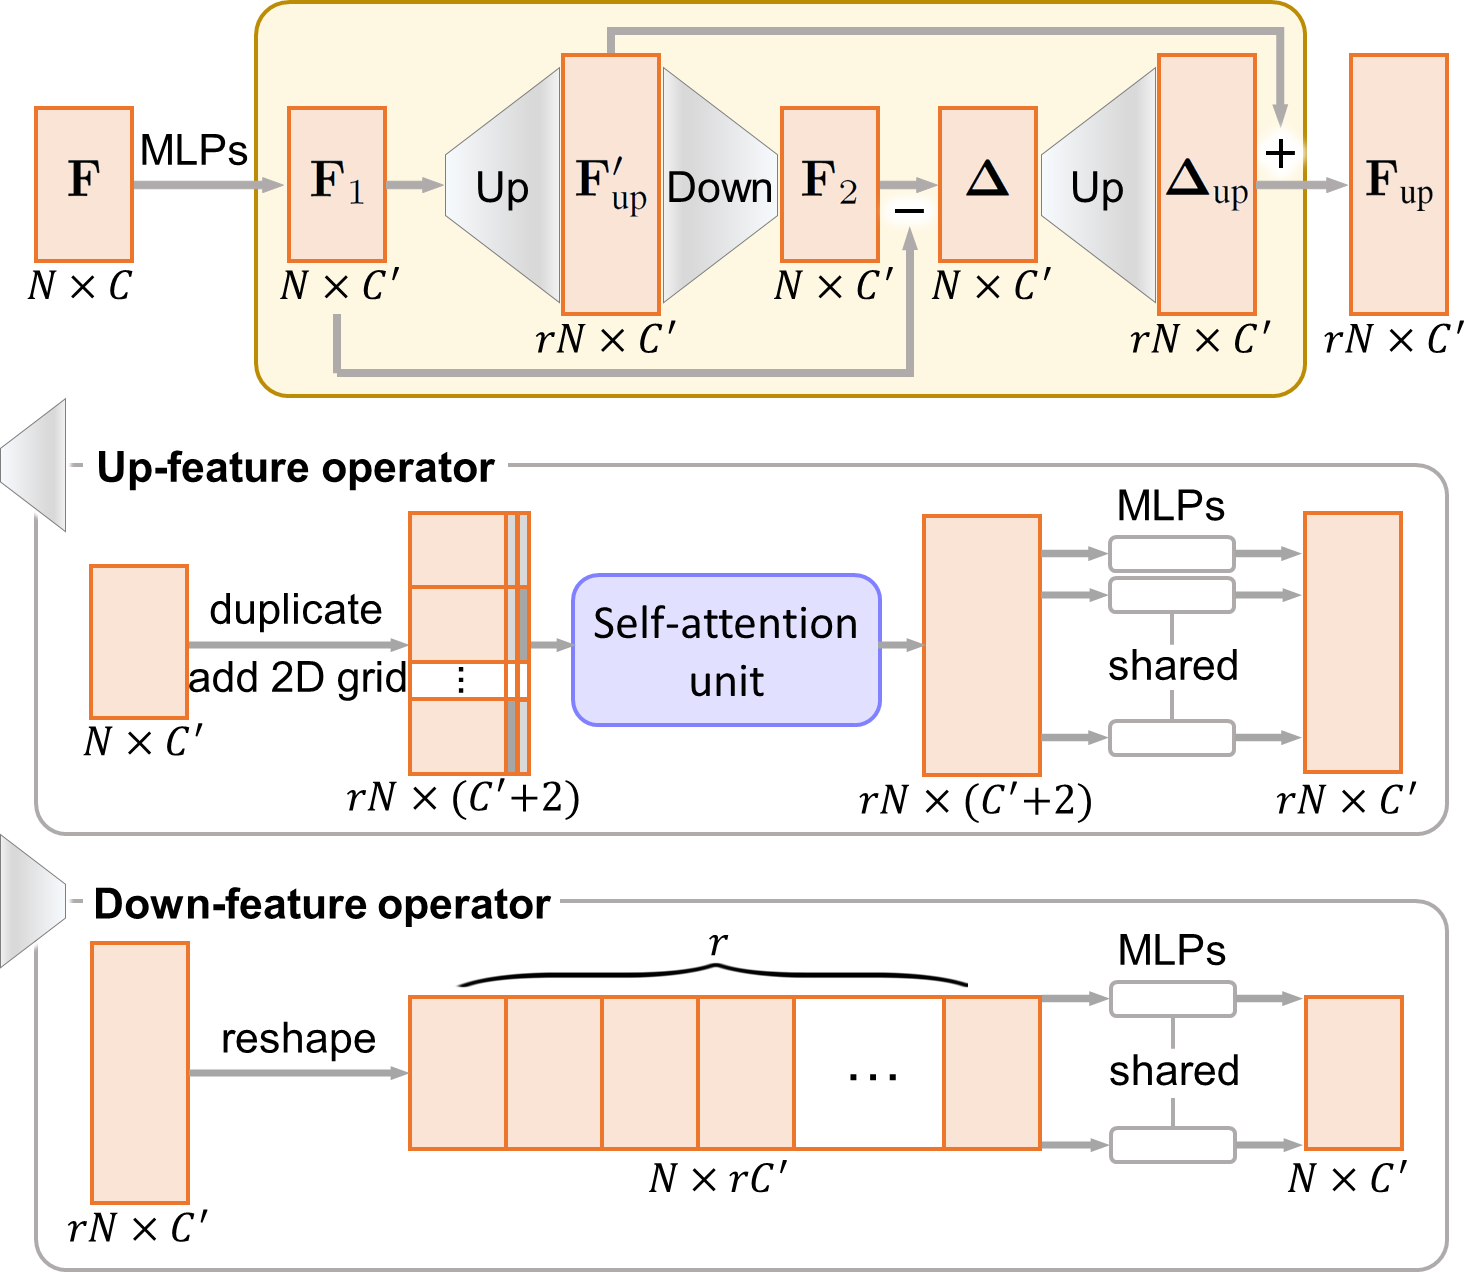
\includegraphics[width=0.98\linewidth]{block}
	\caption{The up-down-up expansion unit (top), up-feature operator (middle), and down-feature operator (bottom).}
	\label{fig:block}
	\vspace*{-2mm}
\end{figure}

%Different from~\cite{yu2018pu} and~\cite{yifan2018patch}
In this work, we construct an up-down-up expansion unit to expand the point features.
To do so, we first upsample the point features (after MLPs) to generate $\mathbf{F}_{\text{up}}^\prime$ and downsample it back (see Figure~\ref{fig:block} (top)); then, we compute the difference (denoted as $\Delta$) between the features before the upsampling and after the downsampling.
By also upsampling $\Delta$ to $\Delta_{\text{up}}$, we add $\Delta_{\text{up}}$ to $\mathbf{F}_{\text{up}}^\prime$ to self-correct the expanded features;
% to $\mathbf{F}_{\text{up}}$;
see again Figure~\ref{fig:block} (top) for the whole procedure.
Such a strategy not only avoids tedious multi-step training, but also facilitates the production of fine-grained features.
%, thus leading to better reconstructions.

%\phil{a bit straightforward, so I commented these:}
%Specifically, this unit consists of the following sequential steps:
%\begin{enumerate}
%	\item MLPs: $\mathbf{F}_1=f_{\text{mlp}}(\mathbf{F})$
%	\item feature up operation: $\mathbf{F}_{\text{up}}^\prime=f_{\text{up}}(\mathbf{F}_1)$,
%	\item feature down operation: $\mathbf{F}_2=f_{\text{down}}(\mathbf{F}_{\text{up}}^\prime)$,
%	\item residual: $\mathbf{\Delta}=\mathbf{F}_2-\mathbf{F}_1$,
%	\item residual up operation: $\mathbf{\Delta}_{\text{up}}=f_{\text{up}}(\mathbf{\Delta})$,
%	\item summation: $\mathbf{F}_{\text{up}}=\mathbf{F}_{\text{up}}^\prime+\mathbf{\Delta}_{\text{up}}$,
%\end{enumerate}
%Note that $f_{\text{mlp}}$ means the MLPs operation, $f_{\text{up}}$ and $f_{\text{down}}$ denote the feature up and down operations, respectively, and will be detailed later.

%From the above sequential steps we can see that, we organize this unit by alternating between upsampled and downsampled features.
%Compared with the feature expansion in one step, like PU-Net, our up-down-up expansion unit can be regarded as a self-correcting %procedure which feeds the upsampling error ($\mathbf{\Delta}$) to the sampling layer and corrects the solution by adding back the %upsampled error ($\mathbf{\Delta}_{\text{up}}$).
%Hence, this enables a more fine-grained expanded feature map, leading to better reconstruction results.
%\phil{it seems that this paragraph has no new contents/information compared to the paragraph before it... can you shorten it OR %remove it?}

%\if 0
%\begin{figure}[t]
%	\centering
%	\includegraphics[width=1.0\linewidth]{imgs/up_down}
%	\caption{The details of our up operation and down operation.}
%	\label{fig:up_down}
%\end{figure}
%\fi

Next, we discuss the up-feature and down-feature operators in the up-down-up expansion unit (see also Figure~\ref{fig:block}):

\para{Up-feature operator.} \
%The goal of the feature up operation is to
To upsample the point features $r$ times, we should increase the variations among the duplicated features.
This is equivalent to pushing the new points away from the input ones.
%
After we duplicate the input feature map (of $N$ feature vectors and $C'$ channels) $r$ times, we adopt the 2D grid mechanism in FoldingNet~\cite{yang2018foldingnet} to generate a unique 2D vector per feature-map copy, and append such vector to each point feature vector in the same feature-map copy; see Figure~\ref{fig:block} (middle).
%
Further, we use the self-attention unit (see Section~\ref{subsec:attention}) followed by a set of MLPs to produce the output upsampled features.

\para{Down-feature operator.} \
To downsample the expanded features, we reshape the features and then use a set of MLPs to regress the original features; see Figure~\ref{fig:block} (bottom).



%feature contents except for these values
%we first duplicate the whole feature map $r$ times.
%Then we generate a 2D grid with $r$ elements. For each element, we duplicate its coordinate $N$ times to form a $N \times 2 $ vector, and then append it to one of duplicated feature vectors; see Figure~\ref{fig:block} (middle). Note that we do not use the value of each element and we just use the coordinate.

%This mechanism is adopted from the code assignment mechanism in FoldingNet~\cite{yang2018foldingnet}, so that each copy of the duplicated feature vector has a 2D coordinate as an unique label. In this way, we can increase the feature variations before feeding the features to the self-attention unit and then the MLPs; see again Figure~\ref{fig:block} (middle). Moreover, to better blend the concatenated latent code, we employ a self-attention unit and then adopt a set of MLPs to generate the upsampled features.
%two values from a 2D grid attached to it like a label.

%Here, the coordinate is selected from a zero-centered $\sqrt{r} \times \sqrt{r}$ (equals to $r$) grid with side length $s=0.2$.
%By using bilinear interpolation between $[-s,s]$, we can obtain two values at each grid position.

% then append coordinates in a 2D grid to each of the $rN$ feature vectors; see Figure~\ref{fig:block} (middle). Here, the random values are generated by ... \phil{how are they created? need one or two sentences here to describe... but please write in a way that others can understrand}
%
%\phil{I really can't follow the details!!!!!!! E.g., what is $n_x$ and $n_y$? you must define every symbol! what is $s$? in what space? no one can really understand!!!}
%To upsample the features $r$ times, we should try to avoid producing new points close to the original points, similar to FoldingNet~\cite{yang2018foldingnet}, we adopt the idea of code assignment by appending a 2D grid to augment the internal representation variation; see Figure~\ref{fig:block} (middle).
%to each copy of the duplicated features
%Specifically, we first generate a zero-centered $n_x \times n_y$ (equals to $r$) grid with side length $s=0.2$.
%By using bilinear inerpolation between $[-s,s]$, we can obtain two values at each grid position.
%We then organize their coordinates into a $r \times 2$ matrix.
%At last, we duplicate each row of the matrix $N$ times and attach it to each copy of the duplicated features.
%Then we duplicate each row of the matrix $N$ times and concatenate it with each copy of the duplicated features.
%We generate the 2D grid by \phil{Please add some details about the grid values}.

%\phil{the word series has the meaning of successive... so, shall we use set instead?}

%
%The goal of the feature down operation is to recover the original feature map with $N \times C^\prime$ from the expanded feature map with $rN \times C^\prime$.
%The process is illustrated in the bottom row of Figure~\ref{fig:block}, where we first reshape the expanded features and then add MLPs to regress the original feature map.



%%%%%%%%%%%%%%%%%%%%%%%%%%%%%%%%%%%%%%%%%%%%%%%%%%%%%%%%%%%

\subsection{Self-attention Unit}
\label{subsec:attention}

\rh{To introduce long-range context dependencies to enhance feature integration after concatenation}, we adopt the self-attention unit~\cite{zhang2019self} in the generator (see Figure~\ref{fig:block} (middle)), as well as in the discriminator (see Figure~\ref{fig:framework} (bottom)).
%\rh{ We employed the self-attention idea ~\cite{zhang2019self} to introduce long-range context dependencies to improve the
%quality of the point features, rather than simply extracting
%per-point features individually.}
%Compared with the basic MLPs, it helps to better combine and integrate features after concatenation.
%
Figure~\ref{fig:attention} presents its architecture.
%
Specifically, we transform the input features into $\mathbf{G}$ and $\mathbf{H}$ via two separate MLPs, and then generate the attention weights $\mathbf{W}$ from $\mathbf{G}$ and $\mathbf{H}$ by
%
\begin{equation}
\mathbf{W} = f_{\text{softmax}}(\mathbf{G}^T \mathbf{H}) \ ,
\end{equation}
%
where $f_{\text{softmax}}$ denotes the softmax function.
After that, we obtain the weighted features $\mathbf{W}^T\mathbf{K}$, where $\mathbf{K}$ is the set of features extracted from the input via another MLP.
Lastly, we generate the output features, which is the sum of the input features and the weighted features.


%\phil{why need MLP before K? How if we remove the bottom-most MLP and K in the attention diagram and multiply W directly with the input features to produce the output features?}
%
%see the ablation study in Section~\ref{subsec:ablation}.
%see an experiment in Section~\ref{sec:experiment}.
%
%This network unit is employed inside both the generator and discriminator networks; see the middle row in Figure~\ref{fig:block} and the bottom row in Figure~\ref{fig:framework}, respectively.

%As we have mentioned above, we add a self-attention unit after the feature concatenation operation inside the feature up operation and the discriminator, respectively.
%Compared with the simple MLPs, this unit can better mix and blend the concatenated features, so that the subsequently extracted features are more expressive.
%Figure~\ref{fig:attention} present the details of the self-attention unit.

%Specifically, the input features are first transformed into two feature space $\mathbf{G}$, $\mathbf{H}$ via MLPs, and the %attention weights $\mathbf{W}$ are calculated by:
%\begin{equation}
%	\mathbf{W} = f_{\text{softmax}}(\mathbf{G}^T \mathbf{H}),
%\end{equation}
%where $f_{\text{softmax}}$ denotes the softmax function.
%Then the output of this attention layer is $\mathbf{W}^T\mathbf{K}$, where $\mathbf{K}$ is the extracted feature map from the %input features via MLPs.

\begin{figure}[!t]
	\centering
	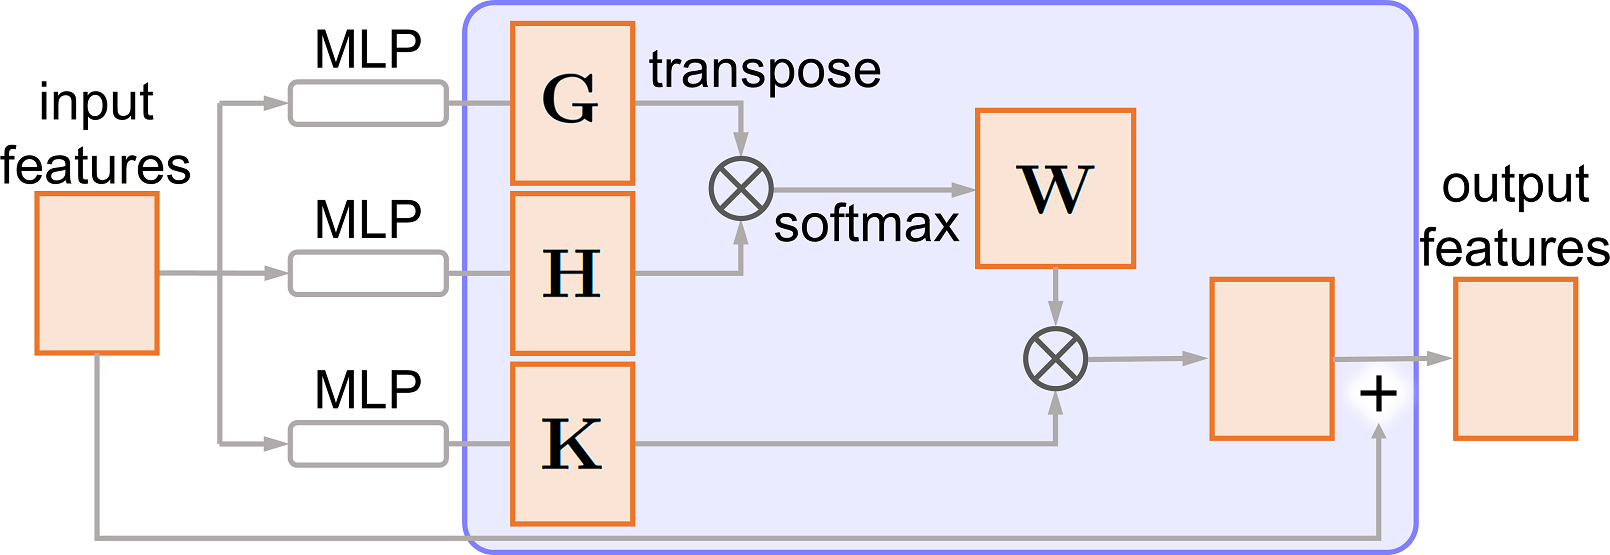
\includegraphics[width=0.75\linewidth]{attention}
	\caption{Illustration of the self-attention unit.}
	\label{fig:attention}
	\vspace*{-2mm}
\end{figure}



%%%%%%%%%%%%%%%%%%%%%%%%%%%%%%%%%%%%%%%%%%%%%%%%%%%%%%%%%%%

\subsection{Patch-based End-to-end Training}
\label{subsec:training}

\subsubsection{Training data preparation}
\label{subsubsec:train_data}

%\phil{after understanding sec 3.5 more, I think we miss an important subsection here to talk about the training and testing dataset, how we produce $\mathbf{P}$ and $\mathbf{\hat{Q}}$, as well as anything that should be done BEFORE the network training}

%\phil{this subsection is to prepare for the data and patches for defining the losses!!!!}

%\phil{So, move Sec 4.1 here and MODIFY... read then modify.. reaad then modify, repeat this at least 3-5 times}

\begin{figure}
	\centering
	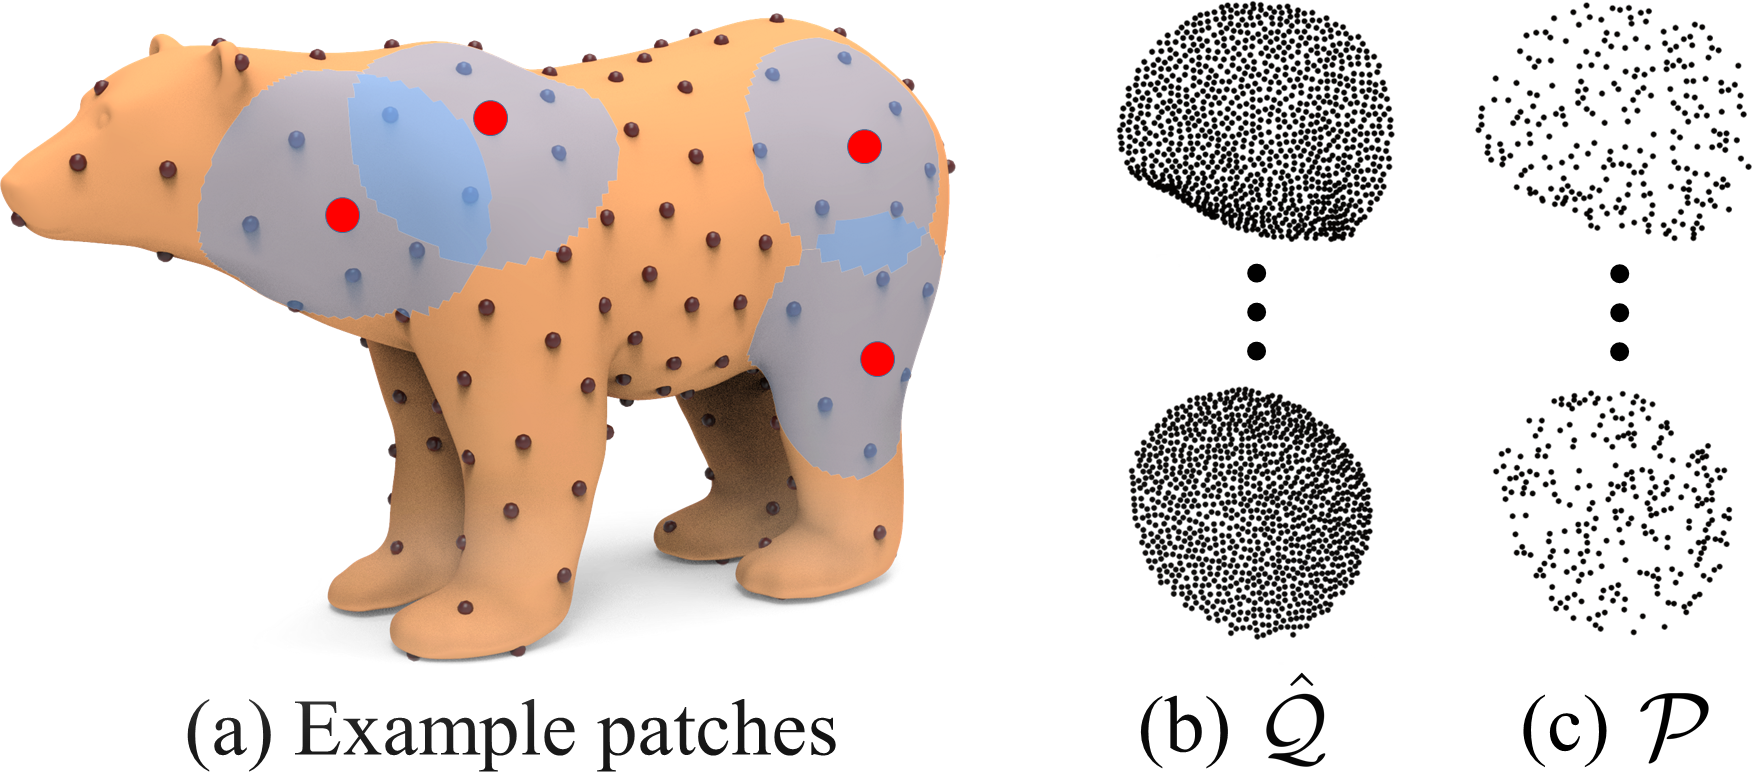
\includegraphics[width=0.9\linewidth]{patch_segment}
	\caption{(a) Seed points (black dots) and patches (blue disks) on a 3D mesh in training data.
(b) \& (c) Example $\mathcal{\hat{Q}}$ and $\mathcal{P}$ on patches.}
%	\caption{Illustration of the training data preparation: (a) we select 200 seed points (black dots) on the object surface and grow a patch (blue circle) at each seed (red dots); (b) we generate a target point set
%$\mathcal{\hat{Q}}$ with $rN$ points on the patch; (c) we generate the network input $\mathcal{P}$ by randomly selecting $N$ points on-the-fly from $\mathcal{\hat{Q}}$.}
	\label{fig:patch_segment}
	\vspace*{-2mm}
\end{figure}

We trained our network to upsample local groups of points over patches on object surface.
%\phil{a small figure to show one or two 3D meshes and a few sample input patches (P) on them?}
%
Specifically, for each 3D mesh (normalized in a unit sphere) in training set (see Section~\ref{subsec:dataset}), we use randomly
%farthest sampling to
find 200 seed positions on each mesh surface, geodesically grow a patch from each seed (each patch occupies $\sim$5\% of the object surface), and then normalize each patch within a unit sphere; see Figure~\ref{fig:patch_segment}(a).
%
On each patch, we further use Poisson disk sampling~\cite{corsini2012efficient} to generate $\mathcal{\hat{Q}}$, which is a target point set of $rN$ points on the patch.
During the training, we generate the network input $\mathcal{P}$ by randomly selecting $N$ points on-the-fly from $\mathcal{\hat{Q}}$.

%%%%%%%%%%%%%%%%%%%%%%%%%%%%%%%%%%%%%%%%%%%%%%%%%%%%%%%%%%%
\subsubsection{Loss functions}
\label{subsubsec:loss}


We now present the compound loss designed for training PU-GAN in an end-to-end fashion.

%In this subsection, we illustrate loss functions that are employed to train our PU-GAN in an end-to-end fashion, which consists of an \emph{adversarial loss}, a \emph{uniform loss} and a \emph{reconstruction loss}.



%%%%%%%%%%%%%%%%%%%%%%%%%%%%%%%%%%%%%%%%%%%%%%

\para{Adversarial loss.} \
%To stabilize our model training procedure and have a high convergence rate,
To train the generator network $G$ and discriminator network $D$ in an adversarial manner, we use the least-squared loss~\cite{mao2017least} as our adversarial loss:
%
\begin{eqnarray}
\mathcal{L}_{\text{gan}}(G)&=&\frac{1}{2}[D(\mathcal{Q})-1]^2 \\
\text{and} \ \
\mathcal{L}_{\text{gan}}(D)&=&\frac{1}{2}[D(\mathcal{Q})^2 + (D(\mathcal{\hat{Q}})-1)^2],
\end{eqnarray}
%
where
%$\mathcal{Q}$ is the generator output;
%$\mathcal{\hat{Q}}$ is the target point set;
%and
$D(\mathcal{Q})$ is the confidence value predicted by $D$ from generator output $\mathcal{Q}$.
%
During the network training, $G$ aims to generate $\mathcal{Q}$ to fool $D$ by minimizing $\mathcal{L}_{\text{gan}}(G)$, while $D$ aims to minimize $\mathcal{L}_{\text{gan}}(D)$ to learn to distinguish $\mathcal{Q}$ from $\mathcal{\hat{Q}}$.
%
%In the training process, $\mathcal{Q}$ and $\mathcal{\hat{Q}}$ need not be paired, and we produce $\mathcal{\hat{Q}}$ by Poisson disk sampling on the underlying object surface.
%\phil{the last sentence here better goes to the new Sec 3.5}
%In the testing process, only the well-trained generator needs to be utilized to reconstruct a point cloud from a sparse input.
%Compared with the traditional logarithmic loss function, we empirically found that the least-squared loss helps produce higher-quality results than to converge the generated data distribution to the decision boundary\cite{zhu2017unpaired},



%%%%%%%%%%%%%%%%%%%%%%%%%%%%%%%%%%%%%%%%%%%%%%

\para{Uniform loss.} \
The problem of learning to generate point sets in 3D is complex with an immense space for exploration during the network training.
Particularly, we aim for uniform distributions; using the adversarial loss alone is hard for the network to converge well.
%making it hard for the network to converge well with the adversarial loss alone.
%making it hard for the network to converge well .
Thus, we formulate a uniform loss to evaluate $\mathcal{Q}$ from the generator, aiming to improve the generative ability of the generator.
% and promote the discriminator to learn more latent patterns.
% from the target distribution.
%
%Only relying on the adversarial loss is not powerful enough, since it is a random and complex procedure to encourage the generator to converge and generate a uniform distribution during training process.
%Hence, to further stabilize and accelerate the convergence of the GAN framework, we formulate a uniform loss in the generator to enhance the distribution uniformity in the generated points, thus promoting the discriminator to discover more latent patterns from the target distribution.

To evaluate a point set's uniformity, the NUC metric in PU-Net~\cite{yu2018pu} crops equal-sized disks on the object surface and counts the number of points in the disks.
So, the metric neglects the local clutter of points.
Figure~\ref{fig:uniformity} shows three patches of points with very different point distributions; since they contain the same number of points, the NUC metric cannot distinguish their distribution uniformity.
%allowing us to evaluate the point distribution uniformity from small local scales to larger global scales.
%the points are whether the points are locally too close to their neighbors.
%since they have the same number of points, their NUC values are the same.
%the three point sets have the same point number, but the distributions are totally different.
%\phil{revise this sentence after Fig.5 is fixed}

\begin{figure}[t]
	\centering
	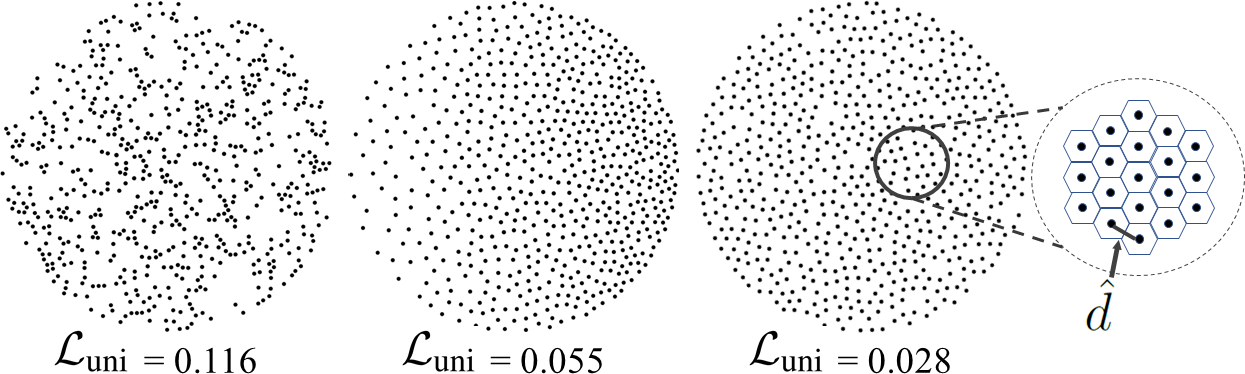
\includegraphics[width=1.0\linewidth]{uniform_example}
	\caption{Example point sets with same number of points (625) but different point distribution patterns; $\mathcal{L_{\text{uni}}}$ is computed with $p$$=$$1\%$.}
%We set $p=1\%$ for uniformity calculation.}
	\label{fig:uniformity}
	\vspace*{-2mm}
\end{figure}

Our method evaluates $\mathcal{Q}$ (a patch of $rN$ points) during the network training by first using the farthest sampling to pick $M$ seed points in $\mathcal{Q}$ and using a ball query of radius $r_d$ to crop a point subset (denoted as $S_j$, $j=1..M$) in $\mathcal{Q}$ at each seed.
Here, we use a small $r_d$, so $S_j$ roughly lies on a small local disk of area $\pi r_d^2$ on the underlying surface.
%
On the other hand, since we form patches by geodesics and normalize them in a unit sphere, patch area is $\sim$$\pi 1^2$.
%generated $\mathcal{Q}$ could be roughly unfolded as a 2D circle with the radius of 1.
%Considering that each training patch $\mathcal{Q}$ is geodesically segmented on the object surface and is normalized within a canonical sphere, each patch thus could be unfolded as a 2D circle with the radius of 1.
So, the expected percentage of points in $S_j$ (denoted as $p$) is $\pi r_d^2 / \pi 1^2 = r_d^2$, and the expected number of points in $S_j$ (denoted as $\hat{n}$) is $rNp$.
%
Hence, we follow the chi-squared model to measure the deviation of $|S_j|$ from $\hat{n}$, and define
%
\begin{equation}
U_{\text{imbalance}}(S_j) = \frac{(|S_j|-\hat{n})^2}{\hat{n}} \ .
\end{equation}

To account for local point clutter, for each point in $S_j$, we find its distance to the nearest neighbor, denoted as $d_{j,k}$ for the $k$-th point in $S_j$.
If $S_j$ has a uniform distribution, the expected point-to-neighbor distance $\hat{d}$ should be roughly $\sqrt{\frac{2\pi r_d^2}{|S_j| \sqrt{3}}}$, which is derived based on the assumption that $S_j$ is flat and neighboring points are hexagonal; see Figure~\ref{fig:uniformity} (right) for an illustration and supplemental material for the derivation.
%
Again, we follow the chi-squared model to measure the deviation of $d_{j,k}$ from $\hat{d}$, and define
%
\begin{equation}
U_{\text{clutter}}(S_j) = \sum_{k=1}^{|S_j|} \frac{(d_{j,k}-\hat{d})^2}{\hat{d}} \ .
\end{equation}
%where $d_{j,k}$ represents the distance between the $k$-th point inside the $j$-th disk and its nearest neighbor.

Here, $U_{\text{clutter}}$ accounts for the local distribution uniformity, while $U_{\text{imbalance}}$ accounts for the nonlocal uniformity to encourage better point coverage.
Putting them together, we formulate the uniform loss as
%
\vspace*{-1.5mm}
\begin{equation}
\label{eq:uniform}
\mathcal{L_{\text{uni}}} = \sum_{j=1}^{M}U_{\text{imbalance}}(S_j) \cdot U_{\text{clutter}}(S_j) \ .
\vspace*{-1mm}
\end{equation}
%
Figure~\ref{fig:uniformity} shows three example point sets with the same number of points but different point distribution patterns.
Using $\mathcal{L_{\text{uni}}}$, we can distinguish the point uniformity among them.
%we can see that, our proposed uniform loss is not only sensitive to local uniformity, but also the global uniformity; see particularly the middle point set.
%


%Then, the area percentage (denoted as $p$) of the local disk over the patch described by $\mathcal{Q}$ can be approximated by $\pi r_d^2/\pi 1^2=r_d^2$.
%with the assumption that the disk is regarded as a 2D circle since it is commonly small enough.
%
%
%We then grow a small disk centered around each seed by using the query ball with the radius of $r_d$.
%Considering that we geodesically \phil{it is wrong to say geodesically here in the training process, right?} crop and normalize each training patch \phil{what exactly is a patch? in methodology, writing should be precise and specific... what is a patch? $\mathcal{Q}$? Never use a term that hasn't been defined clearly in the methodology section}
%within a sphere with radius one, thus the area percentage (denoted as $p$) of the disk over the patch can be calculated \phil{approximated, right?  Another important thing in writing is PRECISION!!!!} by $\pi r_d^2/\pi 1^2=r_d^2$, assuming \phil{..., for small $r_d$.}
%where we approximate both the disk and the patch as 2D circles by considering that the disk is small enough and the patch is geodesically cropped, thus could be unfolded as 2D circles with very few errors.
%\phil{why 1 in the equation? there should be some reasons that you need to explain, right?}
%In our implementation, %instead of a single fixed disk area percentage $p$,
%we obtain multiple small disks around each seed with varying $p$ (\ie, 0.4\%, 0.6\%, 0.8\%, 1.0\%, and 1.2\%).
%For each area percentage $p$, we define $n_j$ as the point number inside the $j$-th disk and $\hat{n}$ as the expected point number for each disk.
%Then, for the $j$-th disk with the number of points as $n_j$, on the one hand,
%If the generated $rN$ points are uniformly-distributed on the patch, the expected point number $\hat{n}$ of each disk can be approximated by $rN \times p$.
%Here, we employ the chi-squared test to measure the imbalance between $n_j$ and $\hat{n}$ given the $j$-th disk, which is denoted as:
%
%\begin{equation}
%	U_{\text{imbalance}}(j) = \frac{(n_j-\hat{n})^2}{\hat{n}}.
%\end{equation}

%On the other hand, if points are uniformly-distributed inside the $j$-th disk of the radius $r_d$ , the expected adjacent point distance $\hat{d}$ can be approximated by $\sqrt{\frac{2\pi r_d^2}{n_j \times \sqrt{3}}}$
%\phil{you MUST prepare a supp. section to derive this number step by step... do it ASAP to make sure that this formulae is correct... I doubt}
%with the assumption that we uniformly split the disk using hexagons of the same size; see the illustration on the rightmost of Figure~\ref{fig:uniformity}.
%Please refer to the supplementary material for the detailed derivation of $\hat{d}$.
%Thus, we formulate the following term to account for the cohesion:
%\begin{equation}
%U_{\text{cohesion}}(j) = \sum_{k=1}^{n_j} \frac{(d_{j,k}-\hat{d})^2}{\hat{d}},
%\end{equation}
%where $d_{j,k}$ represents the distance between the $k$-th point inside the $j$-th disk and its nearest neighbor.

%For the sake of computational efficiency, we design a uniform loss based on a simplified version of the uniformity metric. First, we extract a series of partitions defined as a neighborhood ball in the underlying Euclidean space. To evenly cover the whole surface, the centroids are selected among generated point set by a farthest point sampling (FPS) algorithm. Within our assumption, the normalized patch-based inputs can be regarded as a round surface with a radius 1. Given the size of each neighborhood ball, we can obtain the expected inside number of points $\hat{N}$. In that case, we directly query $\hat{N}$ points for each centroid given a query radius $r$. We will duplicate the centroid point if inside point number is less than $\hat{N}$ and select the nearest $\hat{N}$ point if there are too many point in one ball(whole process is implemented by the ball query ~\cite{qi2017pointnet++}). Finally, the uniform loss is formulated by:

%\begin{equation}
%\mathcal{L_{\text{uni}}} &=& \sum_{D}^{i=0}\sum_{\hat{N}}^{j=0}\left(\frac{(d_{ij}-\hat{d_i})^2}{\hat{d_i}}\right)\\
%\hat{d_i}&=&\sqrt{\frac{2\pi r^2}{\sqrt{3}}}
%\end{equation}
%where $d_{ij}$ represents the distance between $jth$ point and its nearest neighbour and $\hat{d_i}$ is the corresponding expected distance and it will be the same for all balls given a fixed radius.



%%%%%%%%%%%%%%%%%%%%%%%%%%%%%%%%%%%%%%%%%%%%%%

\para{Reconstruction loss.} \
Both the adversarial and uniform losses do not encourage the generated points to lie on the target surface.
Thus, we include a reconstruction loss using the Earth Mover's distance (EMD)~\cite{fan2016point}:
%to emphasize the geometric consistency between the predicted point set and the sampled point set on the surface:
%
\vspace*{-1.5mm}
\begin{equation}
	\mathcal{L_{\text{rec}}} = \min_{\phi:\mathcal{Q}\rightarrow \mathcal{\hat{Q}}} \sum_{q_i\in \mathcal{Q}} \|q_i-\phi(q_i)\|_2,
	\vspace*{-1mm}
\end{equation}
%
where %$\mathcal{\tilde{Q}}$ is a sampled patch of points co-located with $\mathcal{Q}$, simply for representing the underlying object surface, and
$\phi:\mathcal{Q}\rightarrow \mathcal{\hat{Q}}$ is the bijection mapping.



%%%%%%%%%%%%%%%%%%%%%%%%%%%%%%%%%%%%%%%%%%%%%%

\para{Compound loss.} \
Overall, we train PU-GAN end-to-end by minimizing $\mathcal{L}_G$ for generator and  $\mathcal{L}_D$ for discriminator:
\begin{eqnarray}
\label{eq:compound}
	\mathcal{L}_G&=& \lambda_{\text{gan}}\mathcal{L_{\text{gan}}}(G) +\lambda_{\text{rec}}\mathcal{L_{\text{rec}}} + \lambda_{\text{uni}}\mathcal{L_{\text{uni}}}, \\
	\text{and} \ \
    \mathcal{L}_D&=&\mathcal{L}_{\text{gan}}(D),
\end{eqnarray}
where $\lambda_{\text{gan}}$, $\lambda_{\text{rec}}$, and $\lambda_{\text{uni}}$ are weights.
%to balance the relative importance of each loss term.
During the training process, $G$ and $D$ are optimized alternatively.

%why we do not sample centroids on the uniform sample, cause if do so, at the begining, the unform will take a prominent position with a non-uniform outputs, however, we need to be steady to train the nerwork

